% \documentclass[handout,usesnames,table]{beamer}
\documentclass[usenames,table,aspectratio=169]{beamer}

\usepackage[utf8]{inputenc}
\usepackage[spanish]{babel}
\usepackage{xcolor,pgf}% http://ctan.org/pkg/{listings,xcolor,transparent}
\usepackage{pbox}
\usepackage{tikz}
\usepackage{mathabx}
\usepackage{beamerthemeshadow}
\usepackage{times}
\usepackage{enumerate}
\usepackage{graphicx}
\usepackage{graphics}
\usepackage{listings}
\usepackage{multicol}
\usepackage{amsmath,amssymb,amsfonts,latexsym,stmaryrd}
\usepackage{tabularx}
\usepackage{colortbl}
\usepackage{ragged2e} % para justificar texto
\usepackage{textcomp} % Para usar simbolos en texto tipo +- etc
\usepackage{siunitx}
\usepackage{../res/lstlangarm}
\usepackage[absolute,overlay]{textpos}
  \setlength{\TPHorizModule}{1mm}
  \setlength{\TPVertModule}{1mm}
\usepackage{shadow}
\usepackage[many]{tcolorbox}


\usetikzlibrary{calc}
\pgfdeclarelayer{background}
\pgfdeclarelayer{foreground}
\pgfsetlayers{background,main,foreground}


\mode<presentation>{
% 	\usetheme{Warsaw}
% 	\usetheme{Ilmenau}
	\usetheme{Copenhagen}
	\useoutertheme{infolines}
}

\usetikzlibrary{calc}
\pgfdeclarelayer{background}
\pgfdeclarelayer{foreground}
\pgfsetlayers{background,main,foreground}

\newcommand{\IA}{\textsuperscript{\textregistered} 64 }

\setbeamercovered{invisible}

\author{Alejandro Furfaro}
% \title{Organización del Computador II}
% \title{Técnicas Digitales III}
\title{Procesadores ARM - Conmutación de Tareas}
% \institute{Departamento de Computación - FCEyN - UBA}
% \institute{Departamento de Electrónica - UTN.BA}
\date{\today}

\graphicspath
{
	{../img/}
}

\begin{document}


\lstset{
	frame=Ltb,
	framerule=0pt,
	aboveskip=0.5cm,
	framextopmargin=3pt,
	framexbottommargin=3pt,
	framexleftmargin=0.4cm,
	framesep=0pt,
	rulesep=.4pt,
	basicstyle=\small,
	backgroundcolor=\color{gray97}\pgfsetfillopacity{1},
	rulesepcolor=\color{black},
	language=[ARM]Assembler,
	captionpos=b,
	tabsize=6,
	frame=lines,
	keywordstyle=\color{blue},
	commentstyle=\color{purple},
	stringstyle=\color{red},
	numbers=left,
	numberstyle=\tiny,
	numbersep=5pt,
	breaklines=true,
	showstringspaces=false,
	emph={label},
	framerule=0pt,
	xleftmargin=0.4cm,
}

\begin{frame}[plain]{Microprocesadores}
\begin{center}
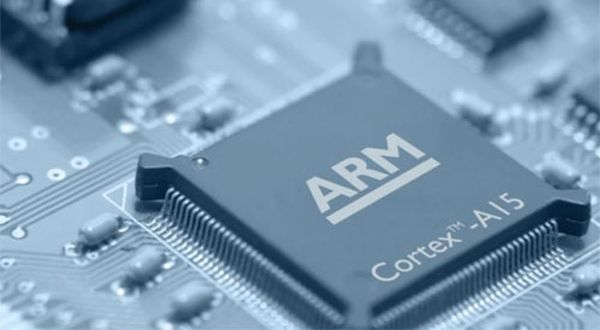
\includegraphics [width =0.4 \textwidth ]{ARM-Cortex.jpg}
\end{center}
\titlepage
\end{frame}

\definecolor{OliveGreen}{RGB}{2,80,1}
\definecolor{LigthOrange}{RGB}{255,255,200}
\definecolor{gray97}{gray}{.97}
\definecolor{Gray}{RGB}{171,174,178}
\definecolor{orange}{RGB}{255,127,0}

\AtBeginSubsection[]
{
\begin{frame}{Temario}
 \begin{textblock*}{\textwidth}(0.4cm,1.4cm)
  \setcounter{tocdepth}{2}  
  \parskip 1cm
  \tableofcontents[currentsection, currentsubsection, sectionstyle=show/shaded, subsectionstyle=show/shaded]
 \end{textblock*}
\end{frame}
}

\begin{frame}{Temario}
 \begin{textblock*}{\textwidth}(0.4cm,1.4cm)
  \parskip 1cm
  \tableofcontents
 \end{textblock*}
\end{frame}


%%%%%%%%%%%%%%%%%%%%%%%%%%%%%%%%%%%%%%%%%%%%%%%%
%Template de aqui en mas ;)
%%%%%%%%%%%%%%%%%%%%%%%%%%%%%%%%%%%%%%%%%%%%%%%%
% \pgfdeclareimage[height=0.9cm]{left-logo}{img/ARM-Cortex.jpg}
% % \pgfdeclareimage[height=0.9cm]{right-logo}{}
% %img/intel-symantec.jpg}
% % \logo{\pgfuseimage{right-logo}}
% \setbeamertemplate{sidebar left}
% {
% \logo{\pgfuseimage{left-logo}}
% \vfill%
% \rlap{\hskip0.1cm\insertlogo}%
% \vskip15pt%
% }
%%%%%%%%%%%%%%%%%%%%%%%%%%%%%%%%%%%%%%%%%%%%%%%%
\definecolor{OliveGreen}{RGB}{2,80,1}
\definecolor{Gray}{RGB}{171,174,178}

\section{Introducción}
\subsection{Conceptos básicos generales}
\begin{frame}{Definiciones}
\begin{textblock*}{\textwidth}(0.4cm,1.2cm)
\begin{description}[<+(1)->] [Espacio de Contexto de ejecución:] \justifying %\parskip 0.3cm
 \item[Tarea:] Unidad de trabajo que un procesador puede despachar, ejecutar, y detener a voluntad, bajo la forma de:
 \begin{itemize} \justifying %\parskip 0.3cm
  \item Instancia de ejecución de un programa (\textit{proceso}, o \textit{thread} para el Sistema Operativo).
  \item Un handler de interrupción, o excepción.
  \item Un servicio del S.O. (por ejemplo en Linux, cualquiera de las Syscall).
 \end{itemize}
% \end{description}
% \end{textblock*}
% \end{frame}

% \begin{frame}{Definiciones}
%  \begin{textblock*}{\textwidth}(0.4cm,1.2cm)
%   \begin{description}[<+(1)->] [Espacio de Contexto de ejecución:] \justifying \parskip 0.3cm 
   \item [Espacio de ejecución:] Es el conjunto de secciones de código, datos, y pila que componen la tarea. 
   \item [Contexto de ejecución:] Es el conjunto de valores de los registros internos del procesador en cada momento. 
   \item [Espacio de Contexto de ejecución:] Bloque de memoria en el que el S.O. almacenará el contexto completo de ejecución del procesador.
  \end{description}
 \end{textblock*}
\end{frame}


\begin{frame}{Context Switch}
 \begin{textblock*}{\textwidth}(0.4cm,1.2cm)
  \begin{block}<1->{Definición} \justifying
Salvar y restaurar el estado computacional o contexto de dos procesos o threads cuando se suspende la ejecución del primero (se salva su contexto) para pasar a ejecutar el segundo (se restaura su contexto). Puede incluir, o no, el resguardo y restauración del espacio de memoria (procesos o threads).
  \end{block}
%  \end{textblock*}
% \end{frame}

% \begin{frame}{Context Switch}
%  \begin{textblock*}{\textwidth}(0.4cm,1.2cm)
  \begin{block}<2->{Primeras conclusiones} \justifying
Las tareas en un computador no operan simultáneamente, sino serialmente pero conmutando de una a otra a gran velocidad. Esto significa que se producen cientos o miles de context switches por segundo.\\
Nuestros sentidos no captan la intermitencia de cada tarea, creándose una sensación de simultaneidad.\\
  \end{block}
 \end{textblock*}
\end{frame}

\begin{frame}{Entra en juego el Sistema Operativo}
 \begin{textblock*}{\textwidth}(0.4cm,1.2cm)
  \begin{itemize}[<+(1)->] \justifying \parskip 0.3cm
   \item En particular, el Sistema Operativo tiene un módulo de software llamado \textbf{\textit{scheduler}}, que trabaja con una lista de tareas a ejecutar.
   \item El \textbf{\textit{scheduler}} define un intervalo de tiempo llamado time frame, el que a su vez con ayuda de un temporizador es dividido en intervalos mas pequeños, que se convierten en la unidad de tiempo.
   \item El arte de manejo de prioridades consiste entonces en asignarle a cada tarea un porcentaje del time frame, medido en una cantidad de intervalos unitarios.
   \item Cada tarea tiene así unos milisegundos para progresar, expirados los cuales suspende una tarea y despacha para su ejecución la siguiente de la lista.
  \end{itemize}
 \end{textblock*}
\end{frame}

\begin{frame}{Integrando lo visto hasta aquí}
 \begin{textblock*}{.95\textwidth}(0.4cm,1.1cm)
  \centering 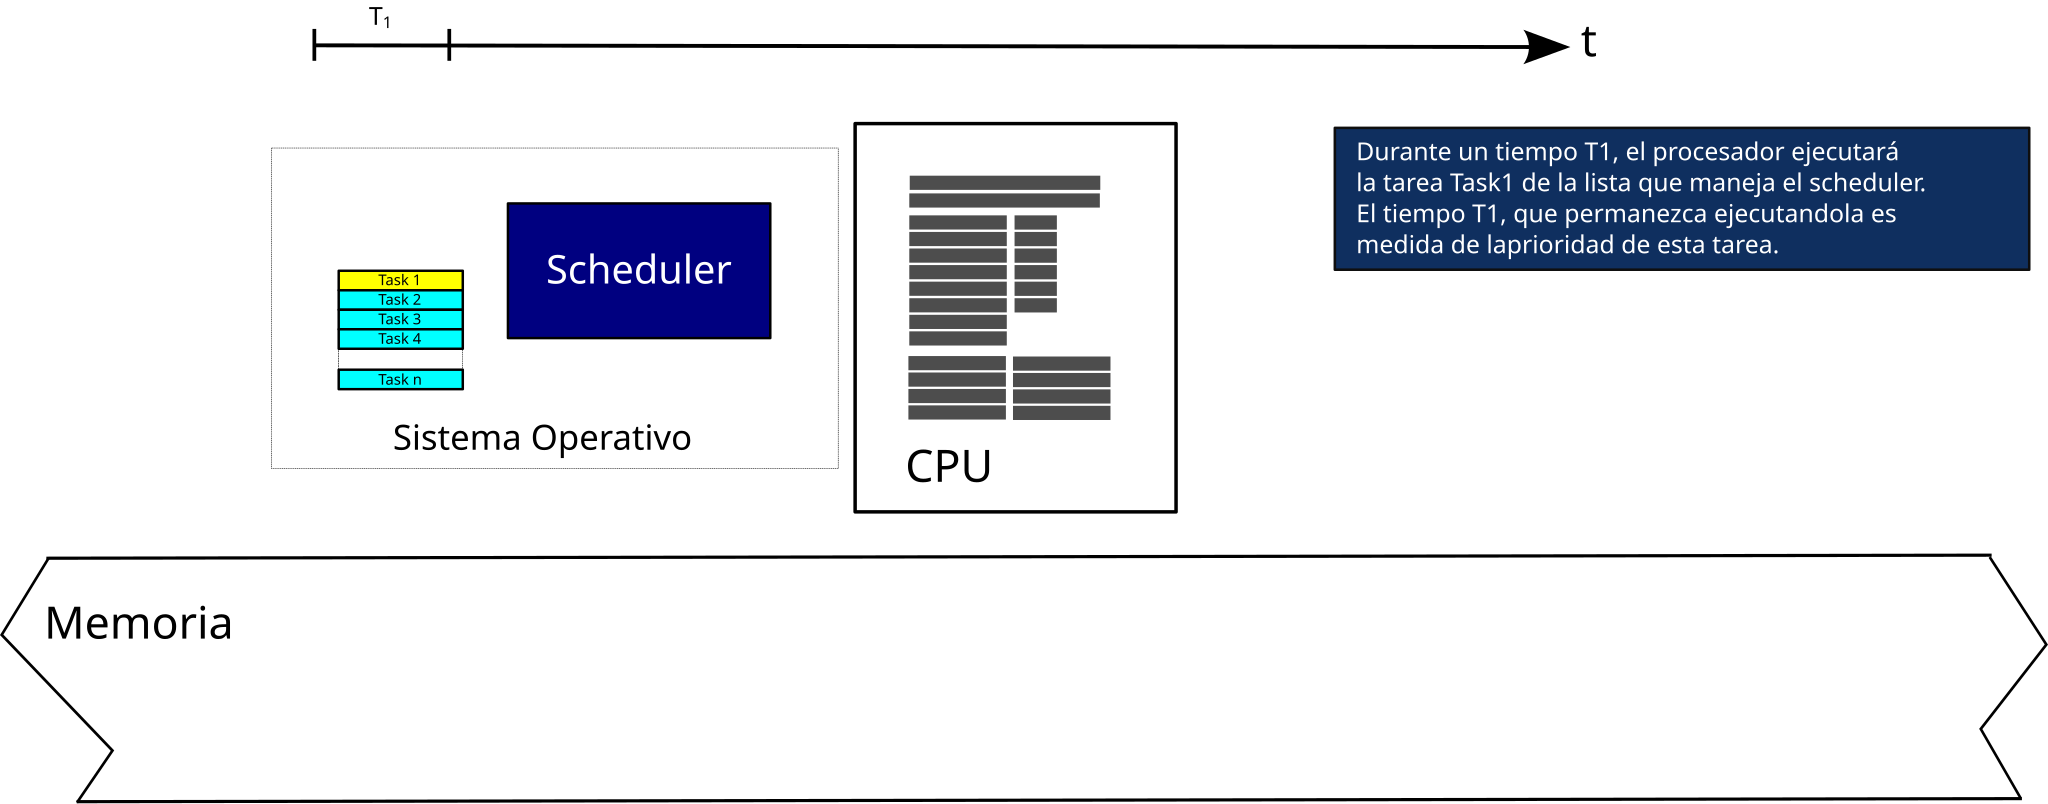
\includegraphics[width=\textwidth]{GenericTaskSwitch1.pdf}\\
 \end{textblock*}
 \begin{textblock*}{\textwidth}(0.4cm,7.1cm)
  \justifying
  \begin{small}
   \only <2->{Durante un tiempo T1, el procesador ejecuta la tarea \textit{Task1} de la lista que maneja el \textbf{\textit{scheduler}}.\\}
   \only <3->{El tiempo T1, que se le asignó para ejecución es medida de la prioridad de esta tarea.}
  \end{small}
 \end{textblock*}
\end{frame}

\begin{frame}{Integrando lo visto hasta aquí}
 \begin{textblock*}{.95\textwidth}(0.4cm,1.1cm)
  \centering 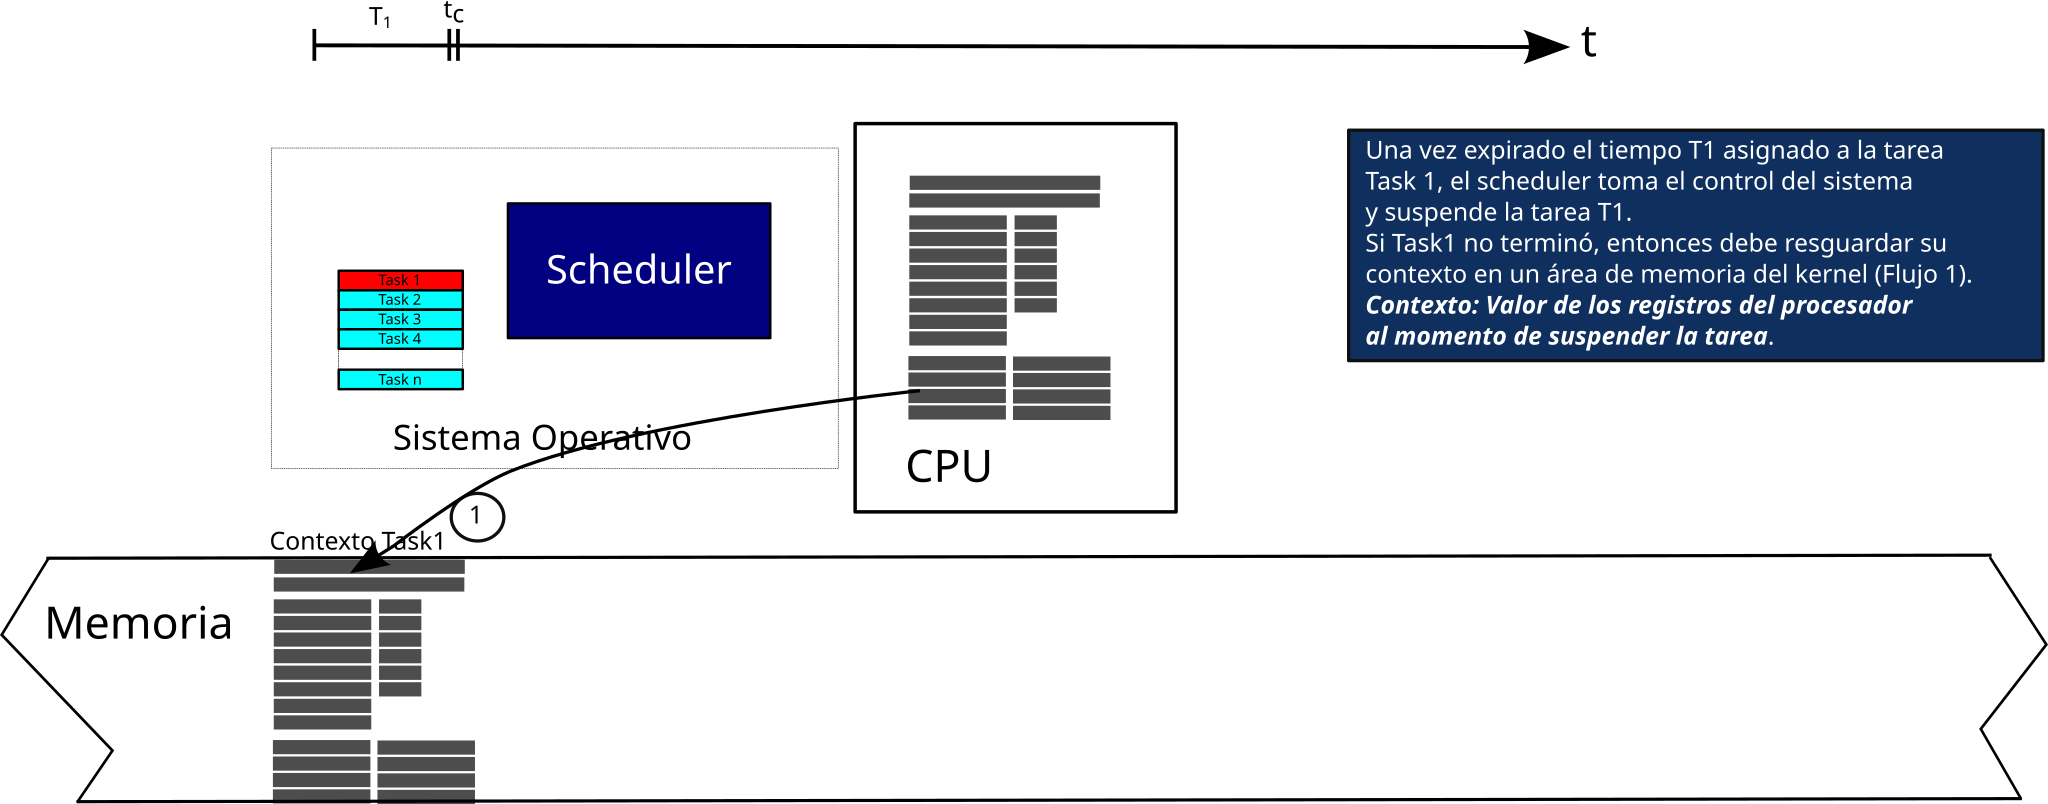
\includegraphics[width=\textwidth]{GenericTaskSwitch2.pdf}\\
 \end{textblock*}
 \begin{textblock*}{\textwidth}(0.4cm,7.1cm)
 \justifying
  \begin{small}
   \only <2->{Una vez expirado T1, el \textbf{\textit{scheduler}} toma el control del sistema y como la tarea \textit{Task1 }no finalizó, la suspende, asignándole estado \textbf{\color{red!90!black}SUSPENDING}.\\}
   \only <3->{Resguarda el contexto de \textit{Task1} en un área de \textbf{memoria del kernel} (Flujo 1).\\}
  \end{small}
 \end{textblock*}
 \begin{textblock*}{.5\textwidth}(5.4cm,5.0cm)
  \only <4->{
   \begin{tcolorbox}[enhanced jigsaw,rounded corners, drop fuzzy shadow=black!50!white]
   \textbf{Contexto: Valor de los registros del procesador al momento de suspender la tarea.}
  \end{tcolorbox}
  }
 \end{textblock*}
\end{frame}

\begin{frame}{Integrando lo visto hasta aquí}
 \begin{textblock*}{.95\textwidth}(0.4cm,1.1cm)
  \centering 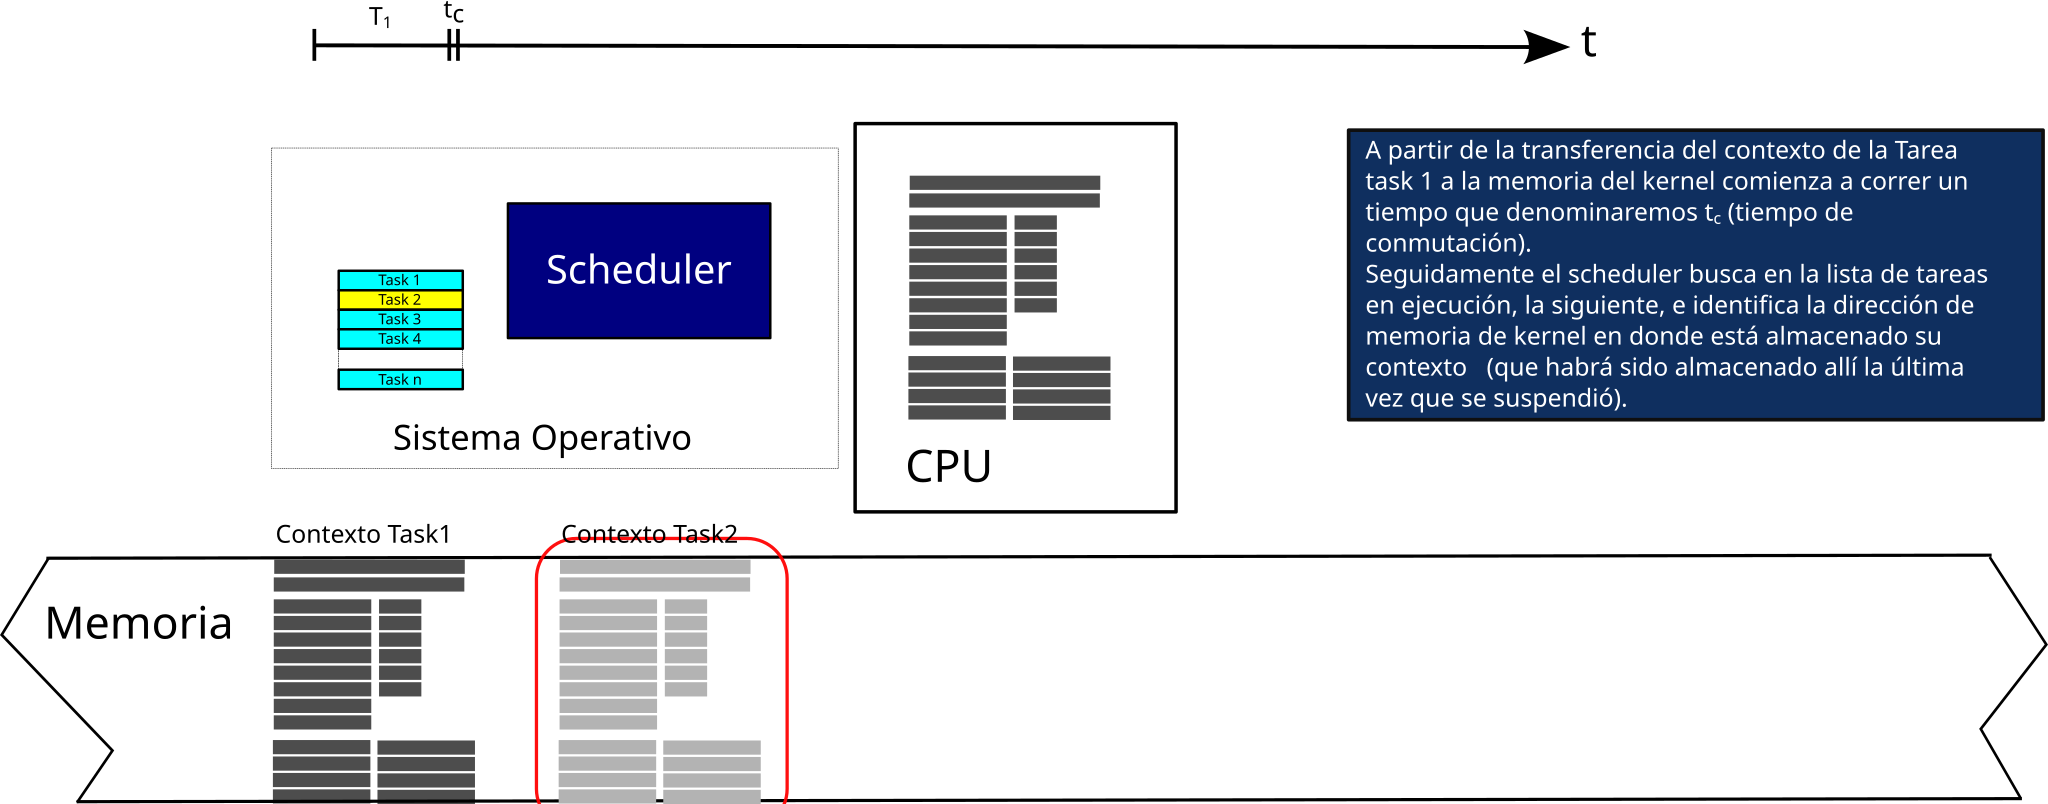
\includegraphics[width=\textwidth]{GenericTaskSwitch3.pdf}\\
 \end{textblock*}
 \begin{textblock*}{\textwidth}(0.4cm,7.1cm)
  \justifying
  \begin{small}
   \only <2>{A partir del inicio de la transferencia del contexto de \textit{Task1} a la \textbf{memoria del kernel} inicia un intervalo que denominaremos $t_{c}$ (tiempo de conmutación).\\}
   \only <3->{Seguidamente el \textbf{\textit{scheduler}} busca la siguiente tarea en la lista de tareas en ejecución (en el gráfico \textit{Task2}), identifica la dirección de memoria de kernel en donde está almacenado su contexto, y marca a la tarea \textbf{\color{yellow!90!red}RUNNING}.}
  \end{small}
 \end{textblock*}
\end{frame}

\begin{frame}{Integrando lo visto hasta aquí}
 \begin{textblock*}{.95\textwidth}(0.4cm,1.1cm)
  \centering 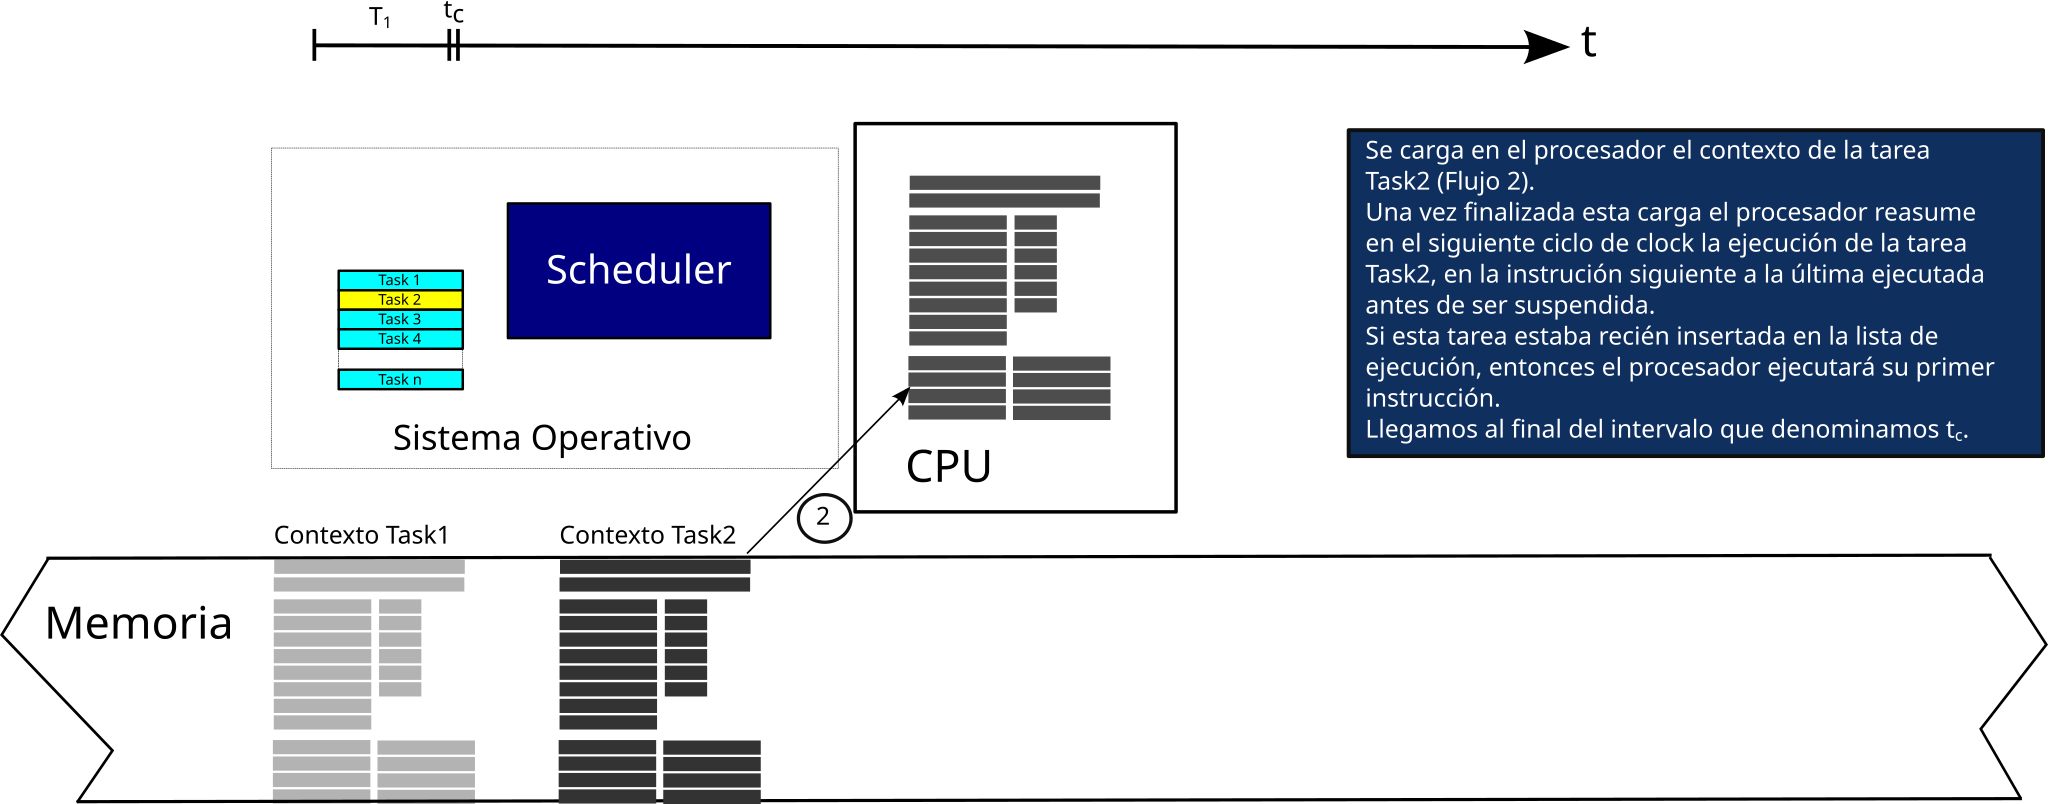
\includegraphics[width=\textwidth]{GenericTaskSwitch4.pdf}\\
 \end{textblock*}
 \begin{textblock*}{\textwidth}(0.4cm,7.1cm)
  \justifying
  \begin{small}
   \only <2-3>{Se carga en el procesador el contexto de la tarea \textit{Task2} (Flujo 2).\\}
   \only <3-3>{En el siguiente ciclo de clock, se reasume la ejecución de \textit{Task2}, en la instrucción siguiente a la última ejecutada antes de ser suspendida.\\}
   \only <4-5>{Si \textit{Task2} fue recién insertada en la lista de ejecución, entonces el procesador ejecutará su primer instrucción.\\}
   \only <5-5>{Llegamos al final del intervalo que denominamos $t_{c}$.}
  \end{small}
 \end{textblock*}
\end{frame}

\begin{frame}{Integrando lo visto hasta aquí}
 \begin{textblock*}{.95\textwidth}(0.4cm,1.1cm)
  \centering 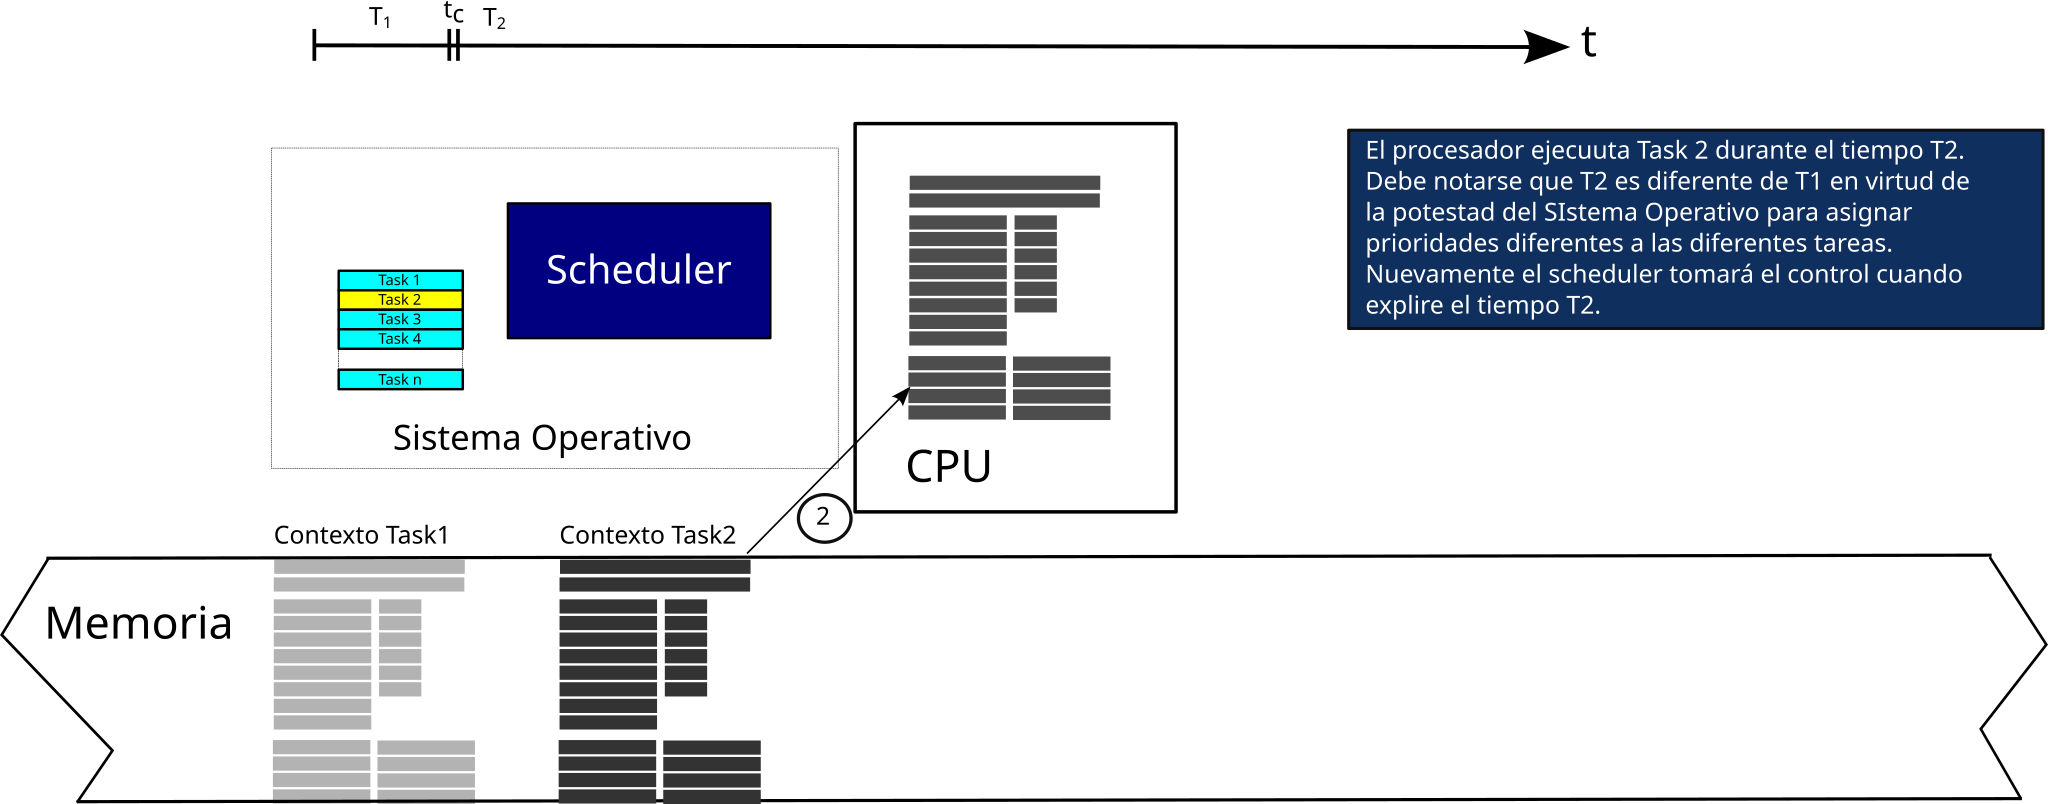
\includegraphics[width=\textwidth]{GenericTaskSwitch5.pdf}\\
 \end{textblock*}
 \begin{textblock*}{\textwidth}(0.4cm,7.1cm)
 \justifying
  \only <2->{El procesador ejecuta \textit{Task2} durante el tiempo T2.\\}
  \only <3->{\underline{\textbf{Nota}}: El Sistema Operativo asigna prioridades diferentes a cada tarea $\therefore T2 != T1$.\\}
  \only <4->{Nuevamente el \textbf{\textit{scheduler}} tomará el control cuando expire el tiempo T2.}
 \end{textblock*}
\end{frame}

\begin{frame}{Integrando lo visto hasta aquí}
 \begin{textblock*}{.95\textwidth}(0.4cm,1.1cm)
  \centering 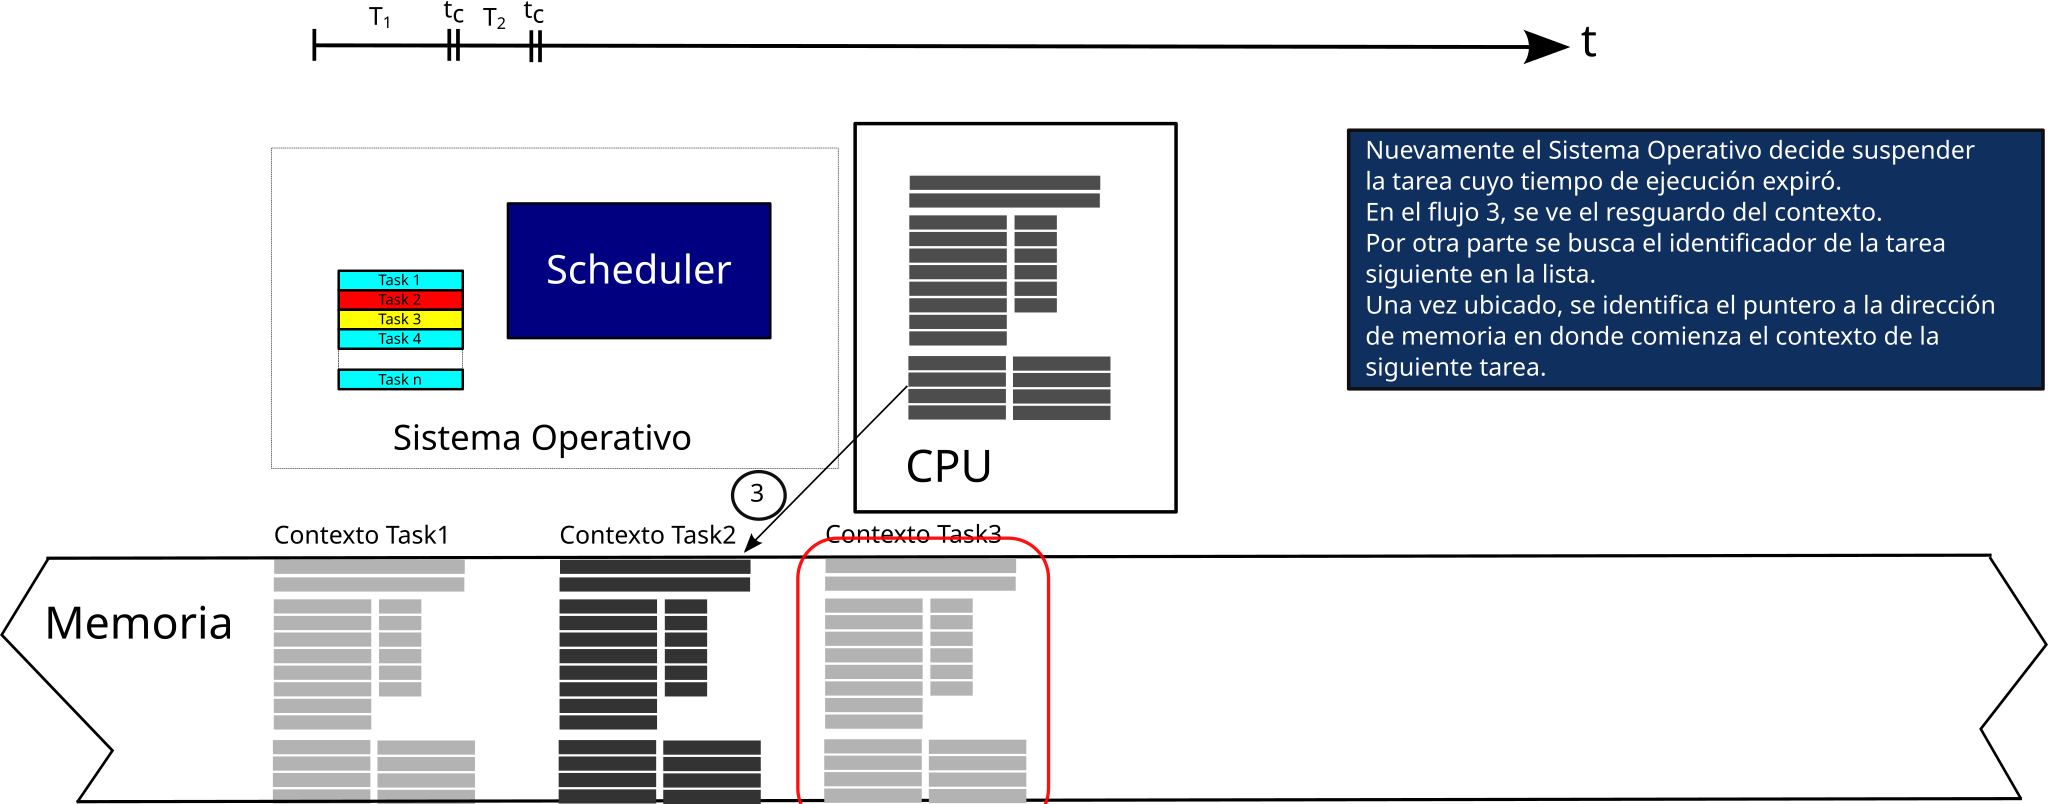
\includegraphics[width=\textwidth]{GenericTaskSwitch6.pdf}\\
 \end{textblock*}
 \begin{textblock*}{\textwidth}(0.4cm,7.1cm)
  \justifying
  \begin{small}
   \only <2-3>{El Sistema Operativo pone \textit{Task2} \textbf{\color{red!90!black}SUSPENDING} ya que su tiempo de ejecución expiró.\\}
   \only <3-3>{En el flujo 3, se ve el resguardo del contexto. Por otra parte se busca el identificador de la tarea siguiente en la lista.\\}
   \only <4->{Una vez ubicado, se identifica el puntero a la dirección de memoria en donde comienza el contexto de la siguiente tarea.}
  \end{small}
 \end{textblock*}
\end{frame}

\begin{frame}{Integrando lo visto hasta aquí}
 \begin{textblock*}{.95\textwidth}(0.4cm,1.1cm)
  \centering 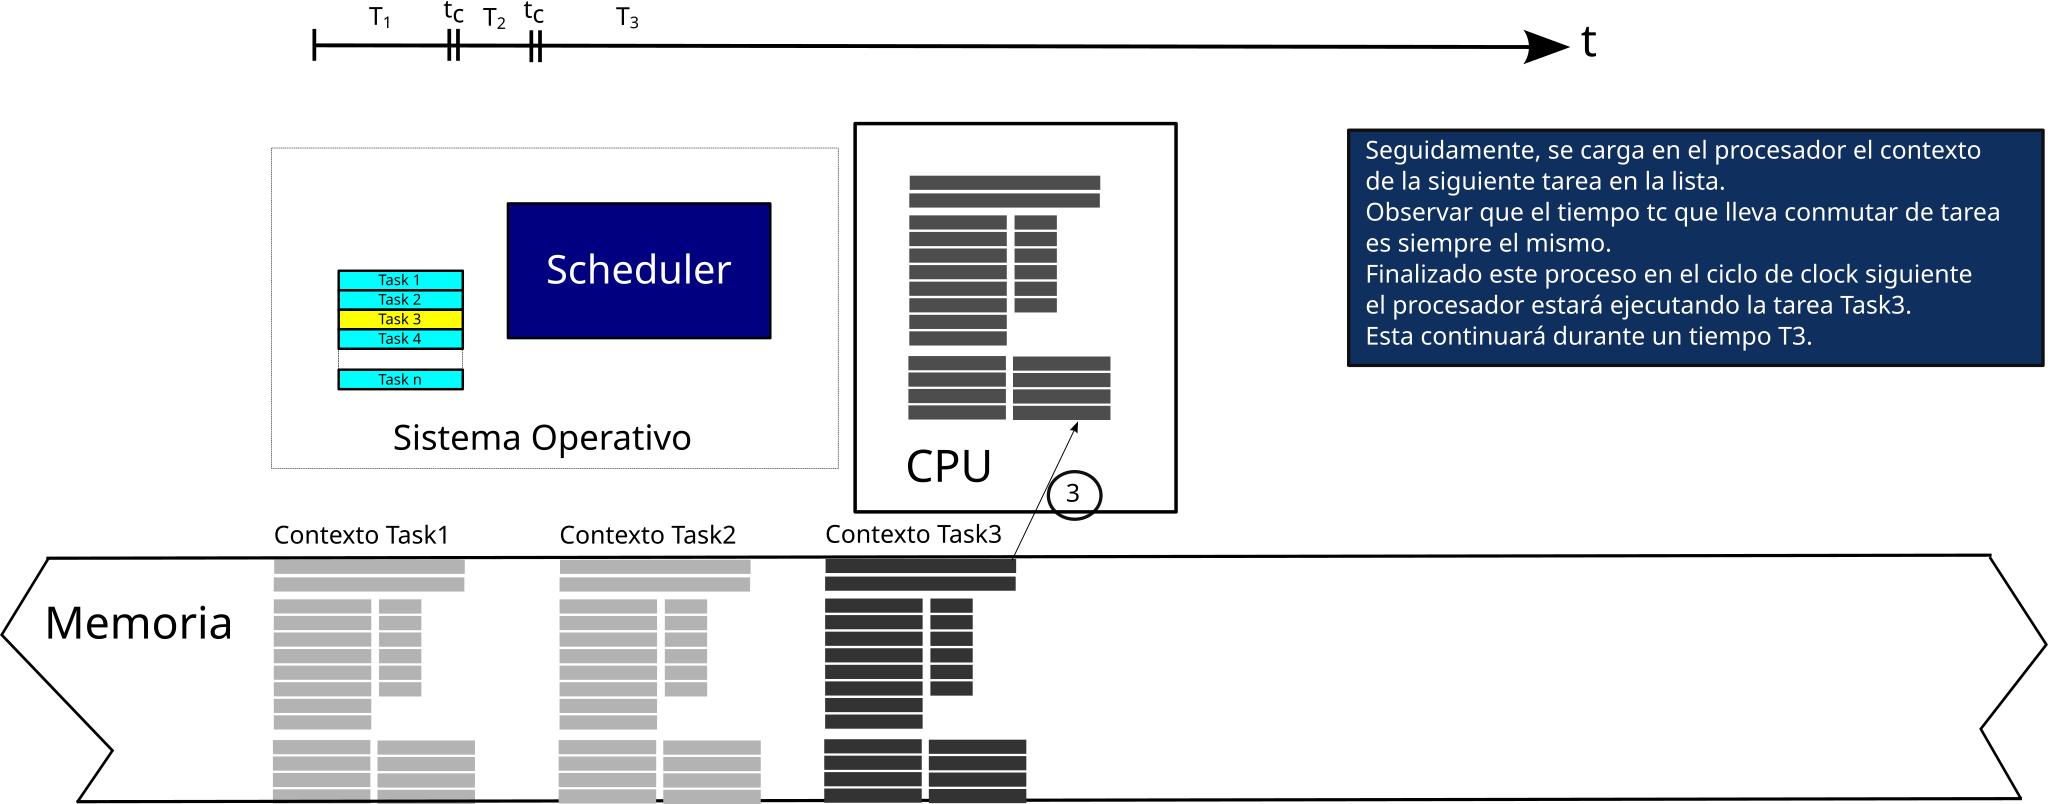
\includegraphics[width=\textwidth]{GenericTaskSwitch7.pdf}\\
 \end{textblock*}
 \begin{textblock*}{\textwidth}(0.4cm,7.1cm)
  \justifying
  \begin{small}
   \only <2-3>{Identificada la tarea siguiente, se carga su contexto en el procesador.\\}
   \only <3-3>{Observar que el tiempo $t_{c}$ es siempre el mismo independientemente de las tareas.\\}
   \only <4-5>{Finalizado este proceso en el ciclo de clock siguiente el procesador estará ejecutando la tarea \textit{Task3}.\\}
   \only <5->{Esta continuará durante un tiempo T3.}  
  \end{small}
\end{textblock*}
\end{frame}

\begin{frame}{Integrando lo visto hasta aquí}
 \begin{textblock*}{.95\textwidth}(0.4cm,1.1cm)
  \centering 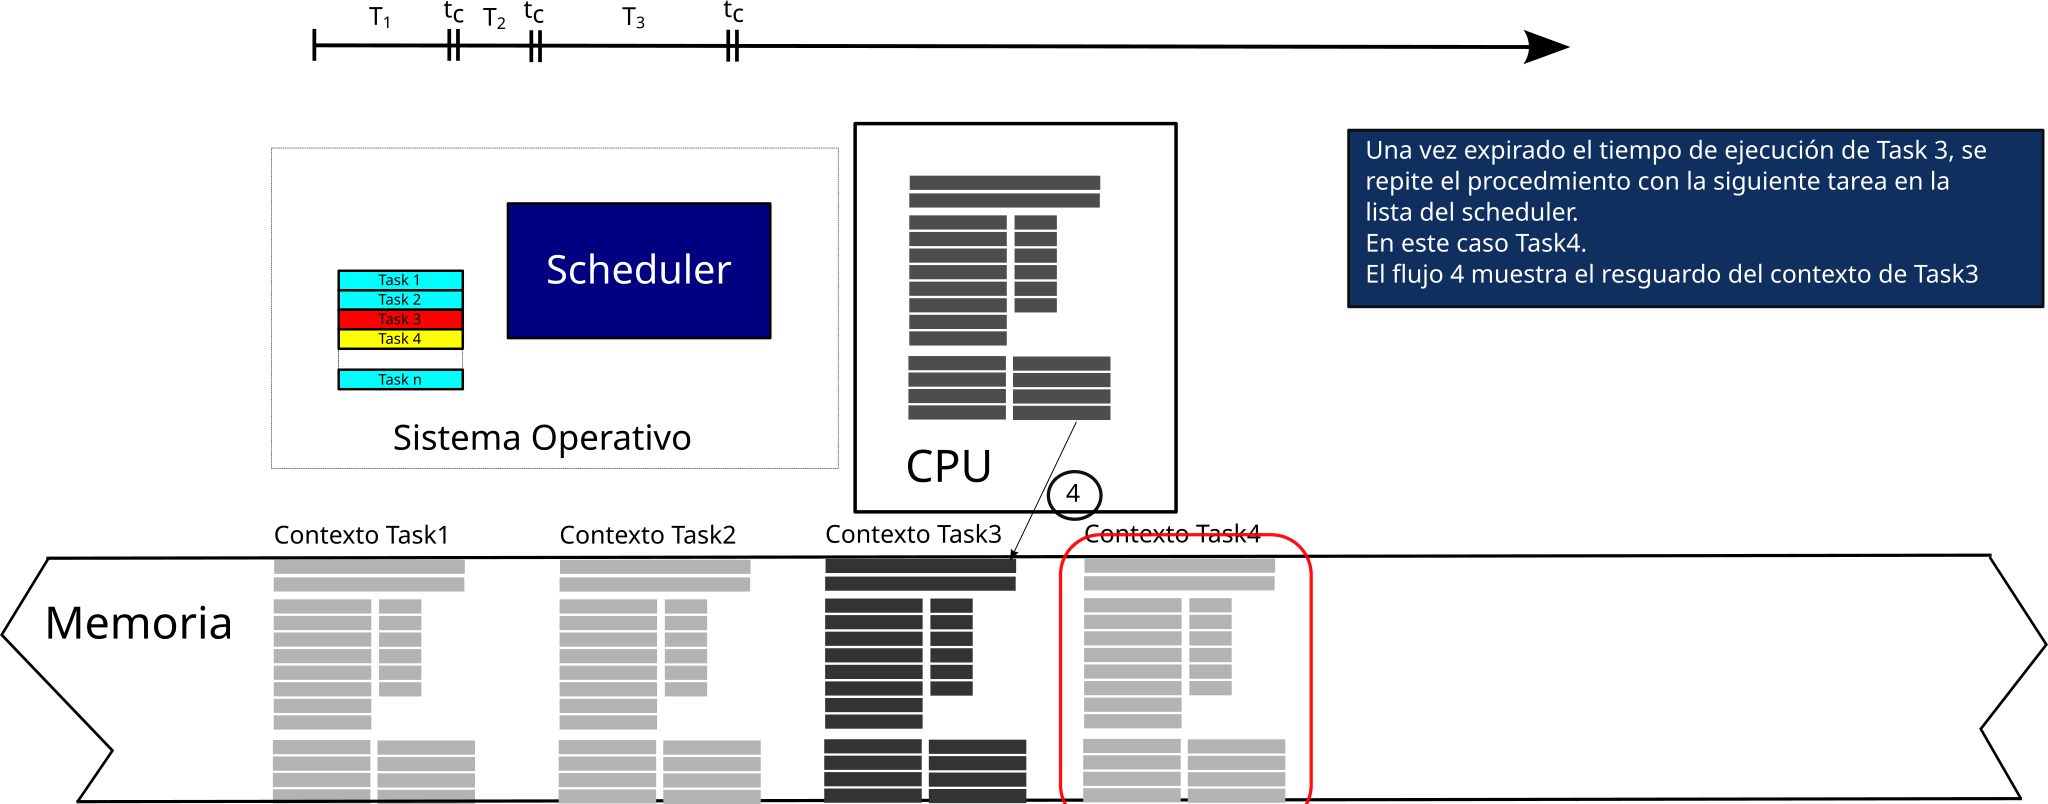
\includegraphics[width=\textwidth]{GenericTaskSwitch8.pdf}\\
 \end{textblock*}
 \begin{textblock*}{\textwidth}(0.4cm,7.1cm)
  \justifying
  \only <2->{Una vez expirado el tiempo de ejecución de \textit{Task3}, se repite el procedimiento con la siguiente tarea en la lista del \textbf{\textit{scheduler}}En este caso \textit{Task4}.\\}
  \only <3->{El flujo 4 muestra el resguardo del contexto de \textit{Task3}.}
 \end{textblock*}
 \end{frame}

\begin{frame}{Integrando lo visto hasta aquí}
 \begin{textblock*}{.95\textwidth}(0.4cm,1.1cm)
  \centering 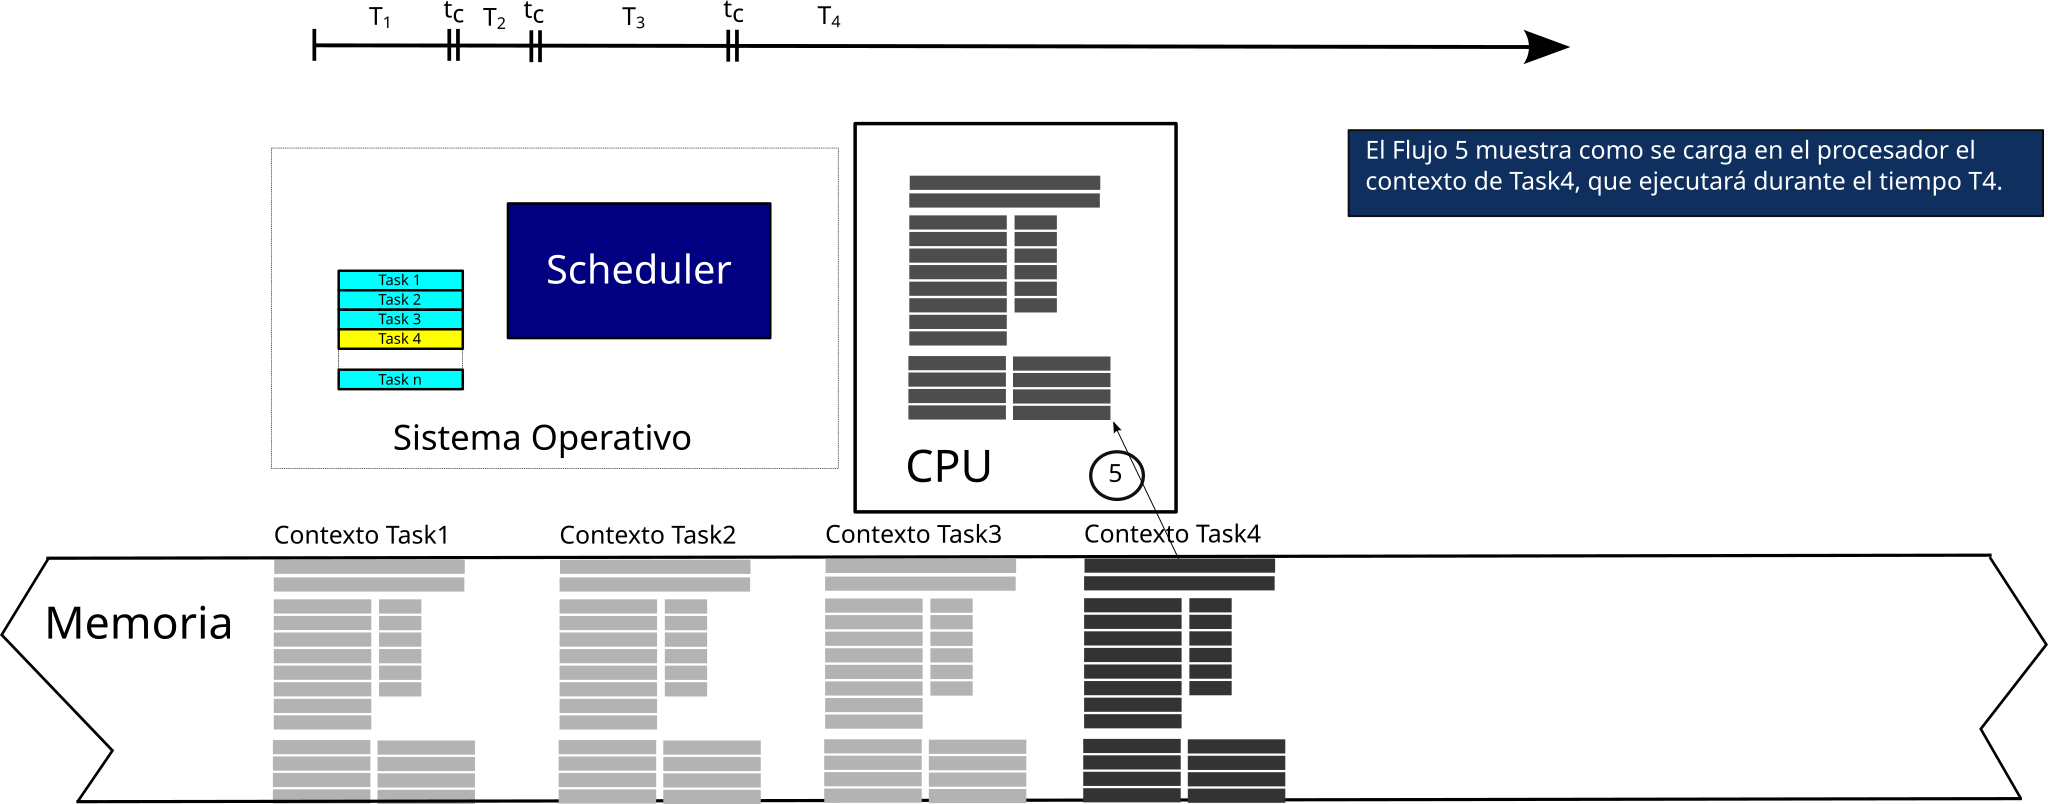
\includegraphics[width=\textwidth]{GenericTaskSwitch9.pdf}\\
 \end{textblock*}
 \begin{textblock*}{\textwidth}(0.4cm,7.1cm) \justifying
  \only <2->{El Flujo 5 muestra como se carga en el procesador el contexto de \textit{Task4}, que ejecutará durante el tiempo T4.}
 \end{textblock*}
\end{frame}

\begin{frame}{Integrando lo visto hasta aquí}
 \begin{textblock*}{.95\textwidth}(0.4cm,1.1cm)
  \centering 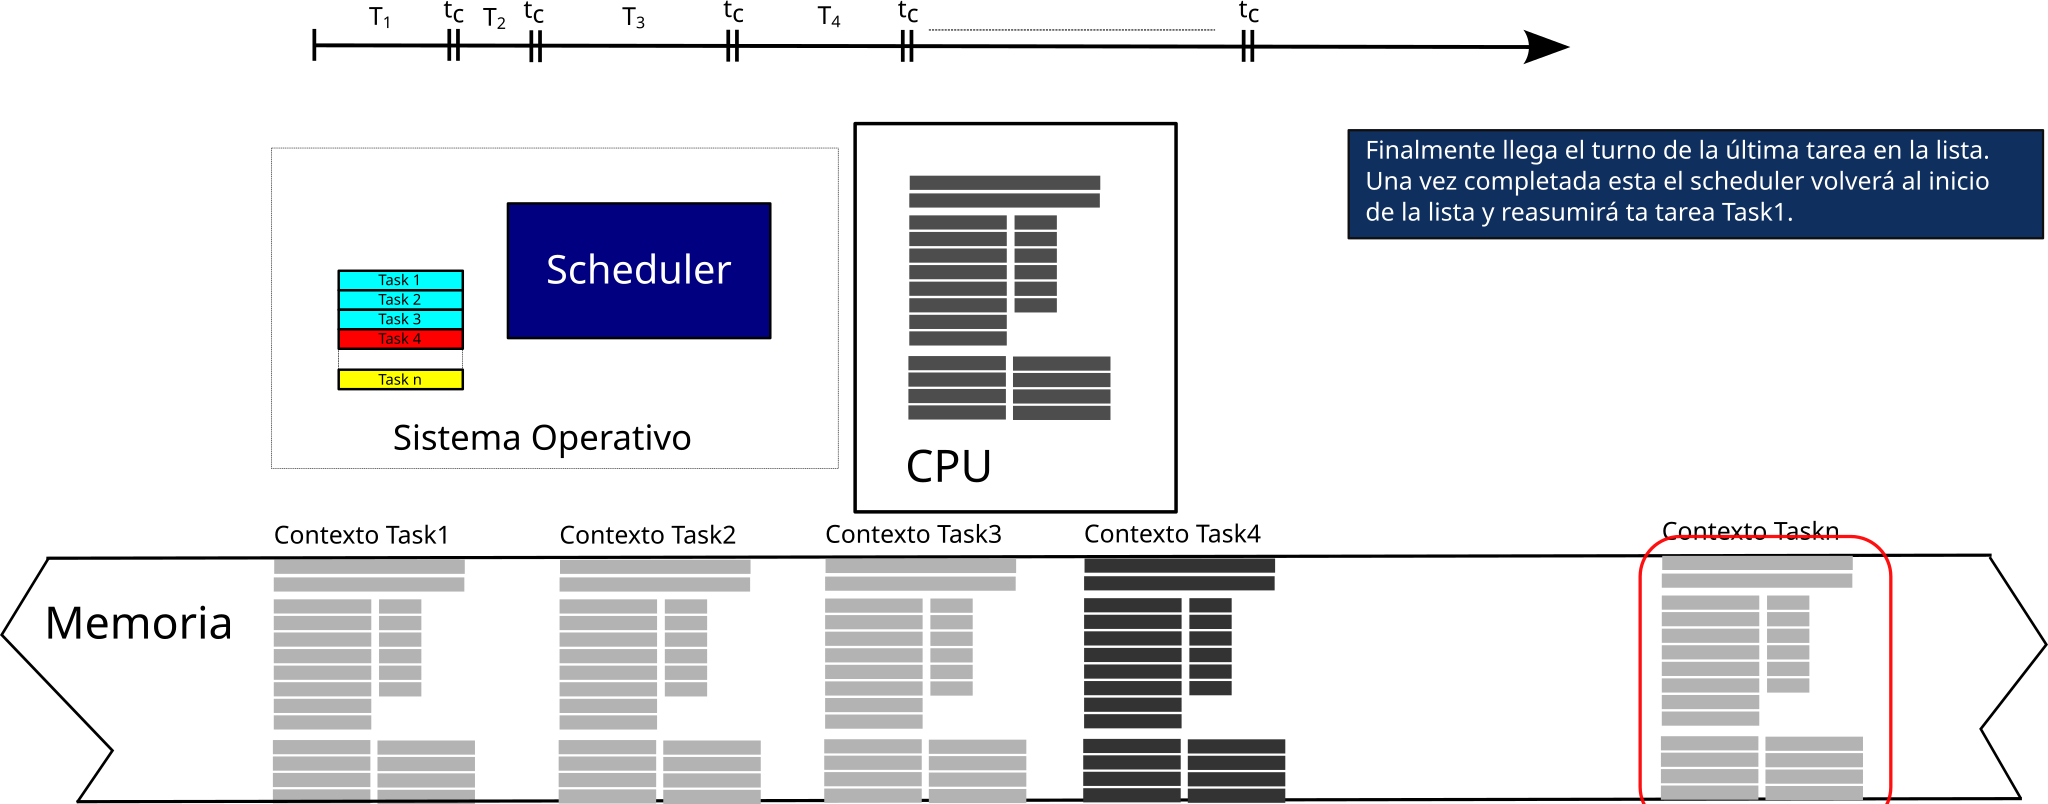
\includegraphics[width=\textwidth]{GenericTaskSwitch10.pdf}\\
 \end{textblock*}
 \begin{textblock*}{\textwidth}(0.4cm,7.1cm)
  \justifying
  \only <2->{Finalmente llega el turno de la última tarea en la lista.\\}
  \only <3->{Una vez completada esta el \textbf{\textit{scheduler}} volverá al inicio de la lista y reasumirá la tarea \textit{Task1}.}
 \end{textblock*}
\end{frame}

\subsection{Modelo de programación de Sistemas Operativos}

\begin{frame}{Modelo de Programación de Sistemas}
 \begin{textblock*}{\textwidth}(0.4cm,1.2cm)
  \begin{itemize}[<+(1)->] \justifying \parskip 0.3cm
   \item Hasta ahora hemos trabajado con la vista de una arquitectura basada en el desarrollo de aplicaciones
   \begin{itemize} \justifying \parskip 0.3cm
    \item [\checkmark] Programación en C, C++, o Assembler en entornos Linux, o Windows.
    \item [\checkmark] Desarrollo de aplicaciones orientadas a objetos en vistosos entornos gráficos.
    \item [\checkmark] Desarrollo de aplicaciones en microcontroladores.
   \end{itemize}
   \item Trabajamos con un conjunto de recursos que se conocen como \textquotedblleft Modelo de programación de Aplicaciones\textquotedblright.
   \item Este modelo describe los registros de propósito general, las instrucciones, los tipo de datos, los modos de direccionamiento\dots tal parece que estaría todo dicho.
   \item Esto no es todo
  \end{itemize}
 \end{textblock*}
\end{frame}

\begin{frame}{¿Acaso hay mas recursos de desarrollo?}
 \begin{textblock*}{\textwidth}(0.4cm,1.2cm)
  \begin{block}<1->{Un paso mas hacia el hardware}
 Si nuestro requerimiento es diseñar un sistema que permita almacenar simultáneamente en memoria varias tareas, administrar su ejecución, evitar que se interfieran, y regular su acceso a los recursos de hardware disponibles, evidentemente estamos entrando en un mundo en el que la visión de Programador de Aplicaciones claramente no es suficiente.
  \end{block}
 \end{textblock*}
\end{frame}

\begin{frame}{¿Acaso hay mas recursos de desarrollo?}
 \begin{textblock*}{\textwidth}(0.4cm,1.2cm)
  \begin{itemize}[<+(1)->] \justifying \parskip 0.3cm
   \item Entonces se trata de desarrollar un conjunto de tareas independientes entre si que contribuyan a implementar el sistema requerido, y un software que las administre.
   \item Necesitamos contar con un SoC cuya CPU tenga capacidades para realizar el propósito planteado.
   \item Si nos las tiene, se puede desarrollar un sistema como el que nos estamos planteando, de todos modos. Pero no esperemos milagros en cuanto a rendimiento, ni le exijamos demasiado al modelo implementado.
   \item Primer paso: tener claro que CPU necesitamos para el requerimiento de nuestro sistema
  \end{itemize}
\end{textblock*}
\end{frame}

\begin{frame}{Modelo de Programación de Sistemas}
 \begin{textblock*}{\textwidth}(0.4cm,1.2cm)
  \begin{itemize}[<+(1)->] \justifying \parskip 0.3cm
   \item El modelo de programación de Aplicaciones de una CPU tiene una visión restringida del sistema en su conjunto.
   \item El modelo de programación de Sistemas, incluye un conjunto de recursos de hardware que amplía la capacidad de la CPU de resolver funciones que le permitan a un Sistema Operativo proveer los servicios y el entorno de programación que \textquotedblleft ven \textquotedblright las aplicaciones, de manera mucho mas veloz y eficiente.
   \item De hecho, el manejo de las excepciones y de las interrupciones de hardware que hemos visto anteriormente es claramente el terreno del Sistema Operativo.
   \item Y hay muchas mas funciones para proveer a un Sistema Operativo desde el hardware que no son necesarias para las aplicaciones.
  \end{itemize}
 \end{textblock*}
\end{frame}

\begin{frame}{Scheduling de Tareas}
 \begin{textblock*}{\textwidth}(0.4cm,1.2cm)
  \begin{itemize}[<+(1)->] \justifying \parskip 0.3cm
   \item Cualquier Sistema Operativo posee un módulo llamado \textbf{scheduler}, que le permite administrar la ejecución de tareas / procesos.
   \item Podemos considerar al \textbf{scheduler} dividido en dos capas: 
   \begin{itemize} \justifying \parskip 0.3cm
    \item [\checkmark]Una de alto nivel en la que se implementan una o mas \textit{políticas} para manejar el cambio de tareas, y que se traducen en diferentes \textit{algoritmos de scheduling}.
    \item [\checkmark]Una de bajo nivel en la que se realiza el \textit{context switch}.
   \end{itemize}
   \item En este punto nos vamos a concentrar en el módulo de \textit{context switch}, dejando para mas adelante los algoritmos de scheduling.
   \item El \textit{context switch} como veremos es físicamente dependiente del procesador y se escribe en assembler.
  \end{itemize}
 \end{textblock*}
\end{frame}

\begin{frame}{Capa de bajo nivel: Context Switch}
 \begin{textblock*}{\textwidth}(0.4cm,1.2cm)
  \begin{itemize}[<+(1)->] \justifying \parskip 0.3cm
   \item Un Context Switch genérico debe llevar a cabo las siguientes acciones:
   \begin{enumerate} \justifying \parskip 0.3cm
    \item Resguardar los registros core y cualquier otro del modelo de programador de aplicaciones en un área de memoria accesible solo para el kernel.
    \item En general el contexto forma parte de una estructura mas amplia llamada genéricamente \textbf{TCB} (por \textbf{T}ask \textbf{C}ontrol \textbf{B}lock) o en la jerga de los sistemas operativos de propósito general PCB (\textbf{P}rocess en lugar de \textbf{T}ask).
    \item Determinar la ubicación del TCB de la siguiente tarea en la lista de tareas en ejecución.
    \item Extraer el contexto de la nueva tarea y copiar registro a registro en la CPU.
   \end{enumerate}
  \end{itemize}
 \end{textblock*}
\end{frame}

\begin{frame}{Capa de alto nivel: Políticas de Scheduling}
 \begin{textblock*}{\textwidth}(0.4cm,1.2cm)
  \begin{itemize}[<+(1)->] \justifying  \parskip 0.3cm
   \item La capa de alto nivel llama al context switch cuando necesita conmutar tareas, en base a criterios definidos en su algoritmo.
   \item Antes de invocar al context switch evalúa una serie de variables:
   \begin{enumerate}
    \item prioridad,
    \item Preemption, 
    \item Atomicidad de operaciones, 
    \item concurrencia, 
    \item limitaciones en tiempo (latency), 
    \item paralelismo (en caso de que el sistema cuente con mas de una CPU), entre otros.
   \end{enumerate}
   \item Por lo tanto un \textbf{scheduler} resulta un código que puede oscilar entre algo muy sencillo, casi trivial, hasta algoritmos muy complejos que puedan considerar los aspectos señalados en el ítem anterior.
  \end{itemize} 
 \end{textblock*}
\end{frame}

\begin{frame}{Conclusiones}
 \begin{textblock*}{\textwidth}(0.4cm,1.2cm)
  \begin{block}<1->{Approach bootom-up} \justifying
  Intentaremos abordar el diseño de un scheduler mas o menos sencillo comenzando por la parte basal: El Context Switch.\\
  Esta es la parte dependiente del hardware. La capa superior interfaz consistente mediante puede reutilizarse, para lo cual es conveniente escribirla en C, para segurar su portabilidad.
  \end{block}
 \end{textblock*}
\end{frame}

\subsection{Cambio de Contexto en Procesadores ARM}

\begin{frame}{Como se resuelve un context switch por Hardware}
 \begin{textblock*}{\textwidth}(0.4cm,1.2cm)
  \begin{itemize}[<+(1)->] \justifying 
   \item En la enorme mayoría de los microprocesadores (y mas aun en los micro controladores) no hay recursos específicos para ayudar a realizar un context switch (también llamado  task switch)
   \item Es decir, que no hay instrucciones específicas ni unidades de hardware que nos ayuden en el context switch.
   \item Resumiendo. ¿Que nos queda?:
  \end{itemize}
 \end{textblock*}
 \begin{textblock*}{\textwidth}(0.4cm,4.3cm)
  \only<5->{\centering 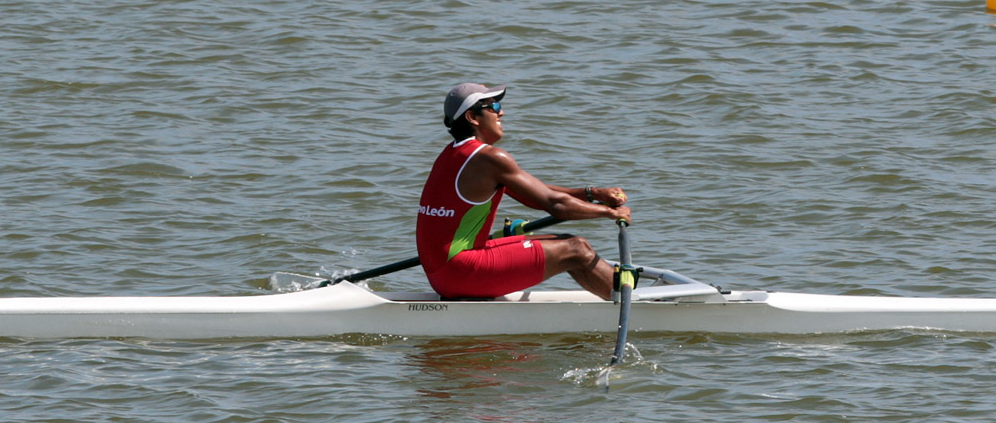
\includegraphics[width=0.66\textwidth]{remarla.png}}
 \end{textblock*}
\end{frame}

\begin{frame}{Como}
 \begin{textblock*}{\textwidth}(0.4cm,1.2cm)
  \begin{itemize}[<+(1)->] \justifying \parskip 0.2cm
   \item La primer pregunta a responder es ¿Como activamos el context switch?
   \item En principio sabemos que activar el context switch es una decisión del \textbf{scheduler} en función de una serie de métricas, y criterios establecidos como políticas en su algoritmo.
   \item El tema es que estas métricas como por ejemplo el tiempo de ejecución de una tarea van cambiando en el tiempo, por lo tanto deben ser monitoreadas de manera regular
   \item Por tal motivo debe implementarse un método para que se active de manera periódica para evaluar las métricas que se hayan definido.
   \item ¿Como?: Respuesta: Usando un timer.
  \end{itemize} 
 \end{textblock*}
\end{frame}


\begin{frame}{Donde}
 \begin{textblock*}{\textwidth}(0.4cm,1.2cm)
  \begin{itemize}[<+(1)->] \justifying \parskip 0.2cm
   \item La siguiente pregunta es ¿Donde ubicamos el código del \textbf{scheduler} entonces?
   \item La respuesta es trivial: En el handler de Interrupción del Timer seleccionado.
   \item Casos prácticos:
   \begin{enumerate}\justifying \parskip 0.2cm  
    \item SYSTICK en los Cortex-M (Recordar que el SYSTICK forma parte de un core CORTEX-M3 en adelante)
    \item El Timer T1 en un SITARA 533x. En la Beagle Bone se utiliza el T1
    \item El Timer T1 del PIT (Programable Interrupt Timer) en cualquier PC IBM compatible, conocido como timer tick
   \end{enumerate}
  \end{itemize}
 \end{textblock*}
\end{frame}

\begin{frame}{Que}
 \begin{textblock*}{.5\textwidth}(0.4cm,1.2cm)
  \begin{itemize}[<+(1)->] \justifying
   \item Siempre se necesita resguardar los registros de propósito general R0-R15, y el CPSR. Pero si están habilitados los coprocesadores...
  \end{itemize}
 \end{textblock*}
 \begin{textblock*}{.5\textwidth}(0.4cm+.5\textwidth,1.2cm)
  \only<3>{\centering \includegraphics[width=0.8\textwidth]{Registers-core.pdf}\\}
  \only<4>{\centering \includegraphics[width=0.8\textwidth]{Registers-core+FPU.pdf}\\}
  \only<5>{\centering \includegraphics[width=0.8\textwidth]{Registers-core+FPU+SIMD.pdf}\\}
  \only<6>{\centering \includegraphics[width=0.8\textwidth]{Registers-core+FPU+SIMD2.pdf}\\}
 \end{textblock*}
\end{frame}

\begin{frame}[fragile]{Guardando los registros del core}
 \begin{textblock*}{\textwidth}(0.4cm,1.2cm)
  \begin{itemize}[<+(1)->] \justifying
   \item Si el scheduler se escribe como handler de una Interrupción, entonces el procesador pasa a ejecutar de modo User a Modo IRQ (no se recomiendo Fast IRQ.
   \item LR recibe el PC+4 (efecto pipeline)
   \item El resto queda tal cual.
   \item El contexto se lleva a la pila y de allí se mueve al \textbf{TCB}.
  \end{itemize}
 \end{textblock*}
 \begin{textblock*}{\textwidth}(0.4cm,4.2cm)
  \begin{onlyenv}<6->
   \begin{lstlisting}
    sub  lr,lr,#4
    push {lr}
    push {r0-r13}
    /*Obtener TCD actual*/
    /*Pasar contexto a TCB actual*/
    /*Obtener el prox. TCB*/
    pop  {r0-r13}
    pop  {pc}
   \end{lstlisting}
  \end{onlyenv}
 \end{textblock*}
\end{frame}

\begin{frame}{Context switch con FPU y SIMD}
 \begin{textblock*}{\textwidth}(0.4cm,1.2cm)
  \begin{itemize}[<+(1)->] \justifying
   \item Como hemos visto solo se debe salvar este contexto para aquellas tareas que lo utilicen, y solo si éste se ha modificado.
   \item De otro modo, si se opta por un approach mas conservador para simplificar el algoritmo de scheduling se está transfiriendo cada vez un bloque de tamaño 5x el de los Registros core.
   \item Nuevamente estamos ante una disyuntiva: \textquestiondown Como podemos comprobar si este contexto cambió?.
   \item Respuesta: No podemos.
   \item \textquestiondown Entonces? \textquestiondown Que hacemos?
  \end{itemize}
 \end{textblock*}
\end{frame}

\begin{frame}{Leer el manual! (nunca falla)}
 \begin{textblock*}{\textwidth}(0.4cm,1.2cm)
  \begin{block}<1->{Del manual de arquitectura Parte B System Level Architecture:} \justifying \scriptsize
\textit{\textbf{B1.11.3. Context switching with the Advanced SIMD and Floating-point Extensions}}\\
In an implementation that includes one or both of the Advanced SIMD and Floating-point Extensions, if the Floating-point registers are used by only a subset of processes, the operating system might implement lazy context switching of the extension registers and extension system registers. In the simplest lazy context switch implementation, the primary context switch software disables the Advanced SIMD and Floating-point Extensions, by disabling access to coprocessors CP10 and CP11 in the Coprocessor Access Control Register, see Enabling Advanced SIMD and floating-point support on page B1-1228. Subsequently, when a process or thread attempts to use an Advanced SIMD or Floating-point nstruction, it triggers an Undefined Instruction exception. The operating system responds by saving and restoring the extension registers and extension system registers. Typically, it then re-executes the Advanced SIMD or Floating-point instruction that generated the Undefined Instruction exception.
  \end{block}
 \end{textblock*}
\end{frame}

\begin{frame}{Bienvenidos al modelo de Programación de Sistemas}
 \begin{textblock*}{\textwidth}(0.4cm,1.1cm)
  \begin{block}<2->{CPACR, Coprocessor Access Control Register, VMSA}  \justifying
En este registro solo accesible en modo privilegiado mediante las instrucciones de acceso a este tipo de registros se puede activar / desactivar los Coprocesadores cp10 (VFP) y cp11 (SIMD)
  \end{block}
 \end{textblock*}
 \begin{textblock*}{\textwidth}(0.4cm,3.9cm)
  \only<3>{\centering \includegraphics[width=\textwidth]{CPACR-layer1.pdf}\\}
  \only<4->{\centering \includegraphics[width=\textwidth]{CPACR-layer2.pdf}\\}
 \end{textblock*}
 \begin{textblock*}{\textwidth}(2.4cm,5.7cm)
  \begin{onlyenv}<5->
   \begin{center}
   \small
    \begin{tabular}{| l | l |}
     valor & Acción \\
     \hline
     {\color{red}00} & {\color{red}Acceso Denegado. Genera Undefined Instruction Exception}.\\
     01 & Acceso en Modo Privilegiado solamente\\
     10 & Reservado\\
     11 & Acceso en Modo Privilegiado y User\\
    \end{tabular}
   \end{center}
  \end{onlyenv}
 \end{textblock*}
\end{frame}

\begin{frame}[fragile]{Acceso al CPACR}
 \begin{textblock*}{\textwidth}(0.4cm,1.6cm)
  \begin{lstlisting}[basicstyle=\footnotesize,]
MRC p15, 0, <Rt>, c1, c0, 2 ; Lee CPACR en el reg. core Rt
MCR p15, 0, <Rt>, c1, c0, 2 ; Escribe Rt en CPACR
  \end{lstlisting}
 \end{textblock*}
 \begin{textblock*}{\textwidth}(0.4cm,3.0cm)
  \begin{itemize}[<+(1)->] \justifying
   \item El registro CAPCR se lee desde el registro de control del Coprocesador 15. 
   \item En este Copropcesador se habilitan las funciones mas importantes del sistema, incluido el acceso a los Coprocesadores CP0 a CP13.
   \item Con este par de instrucciones se habilita o deshabilitan los Corpocesadores CP10 y CP11 que en este caso nos interesa.
  \end{itemize}
 \end{textblock*}
\end{frame}

\begin{frame}{Lazy FPU Context Switch}
 \begin{textblock*}{\textwidth}(0.4cm,1.2cm)
  \begin{itemize}[<+(1)->] \justifying
   \item Se implementa en el Handler de Undefined Instruction Exception.
   \item El truco consiste en tener CP10 y CP11 deshabilitados
   \item Cuando el procesador fetchea una instrucción y al decodificarla la identifica como SIMD o como una operación de la VFP, intenta derivarla a esas unidades. 
   \item Si éstos coprocesadores no están habilitados generará una Excepción Undefined Instruction.
   \item El handler analizará la causa de la falta, y si corresponde a estas instrucciones, habilitará los coprocesadores, busque el tcb de la tarea actual en el cual deberá haber un puntero no nulo a una estructura especial que contendrá todos los registros de punto flotante y SIMD y los cargará en los registros del procesador.
   \item Eventualmente mantendrá un estado (un flag global por ejemplo) para que el scheduler al suspender la tarea guarde el contexto VFP / SIMD e inactive ambos coprocesadores antes de switchear a la siguiente tarea
  \end{itemize}
 \end{textblock*}
\end{frame}

\begin{frame}{Conclusiones}
 \begin{textblock*}{\textwidth}(0.4cm,1.2cm)
  \begin{itemize}[<+(1)->] \justifying
   \item No estamos desarrollando una aplicación, sino un sistema.
   \item Cada funcionalidad relevante, o evento significativo, lleva asociada una tarea.
   \item Se necesita un sistema capaz de administrar la ejecución de estas tareas y su acceso a los recursos
   \item Nos hemos basado mayormente en Cortex-A. 
   \item No obstante, Cortex-M entra en el mundo de la FPU a partir de M4. Con modelos mas reducidos pero conceptualmente similares.
  \end{itemize}
 \end{textblock*}
\end{frame}




\end{document}
